\chapter{Edge Offloading \& Early Exiting}

Early exiting model have been used for two purposes in literature.

\begin{enumerate}
	\item Reducing average inference latency and power consumption by letting samples prematurely exit the model based on random distributions \cite{bibid} or samples passing a threshold measure of confidence \cite{teerapittayanon_branchynet:_2016}.
	\item Comply with application time constraints by exit selection or sub-model selection. By only inference samples up to a selected exit possible to meet stringent delay constraints and reduce waste of computation \cite{li_edge_2018}. 
\end{enumerate}

We have too shown the possibility of 1. to reduce average latency by a early exiting model in section \ref{}. We have also shown, the possibility of adhering to a time constraint, whilst maximizing the accuracy in section \ref{}. This we have shown purely in a lab setup, where no actual offloading takes place. 

Edgent \cite{li_edge_2018} is to our knowledge the only proposal in current literature, that uses early exiting models in an offloading scenario. Edgent combines early exiting and network splitting to handle the accuracy-latency trade-off, by an optimization framework of \gls{dnn} right-sizing and splitting for device-edge collaboration. The optimization done based on regression models of the per layer execution time of the \gls{dnn}. The downside of edgent is an upfront selection of exit i.e gls{dnn} right-sizing, which can be troublesome with unpredictable communication delays. 

We propose a more flexible edge offloading scheme, compared to upfront exit selection. We argue, that allowing the edge server to reach as far as possible, within the time budget and continuously sending back increasingly confident predictions, will in any case achieve at least the same accuracy. Even though a sub-model exit have been chosen with care e.g. using \gls{dnn} right-sizing, the risk of timeout is still present as both computation and communication delays are not constant. If unexpected delays do occur, it may cause timeouts and lead to lost predictions. However, our scheme reduces the risk of losing prediction by timeout, if an earlier, albeit less accurate predictions is available. 

Figure \ref{fig:offloading-scheme} illustrates the offloading scheme. To not waste idle time on edge server the data is offloaded from the end device, to edge server as soon as acquired. The edge server preprocesses the data, runs the \gls{dnn} inference process, and whenever a prediction is obtained from the early ecit \gls{dnn}, a thread is spawned to send back the result to the end device. The end device then decides the prediction based upon the information received from the edge server. Figure \ref{fig:offloading-scheme-successful} illustrates the continuous reply of predictions. Figure \ref{fig:offloading-scheme-timeout} illustrates a case, where a timeout occurs and only two predictions are available.

What about lost prediction? Should we have small model running on end?

Or collaboratively?

We send back top-5 to allow info-combination, since almost always the correct is within these 5 prediction. 

\begin{figure}
	\captionsetup[subfigure]{justification=centering}
	\subfloat[Continuois predictions\label{fig:offloading-scheme-successful}]{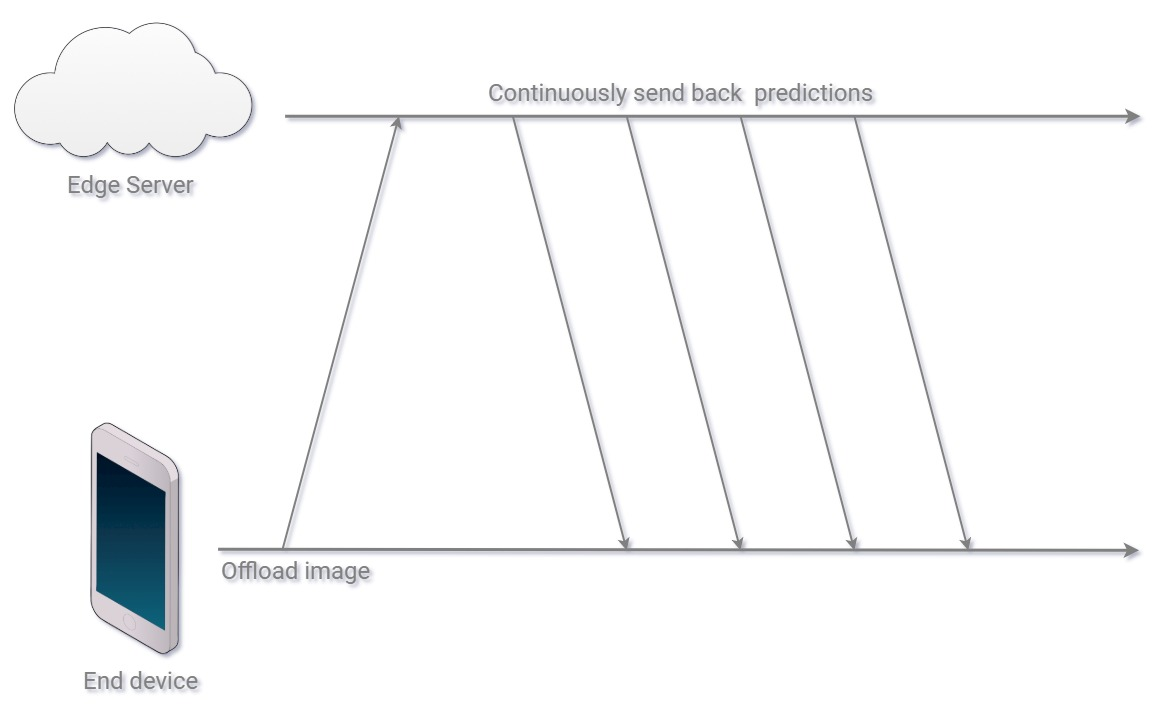
\includegraphics[width=\linewidth]{figures/models/timeline_all}}
	\hfill
	\subfloat[Timeout of Continuois predictions\label{fig:offloading-scheme-timeout}]{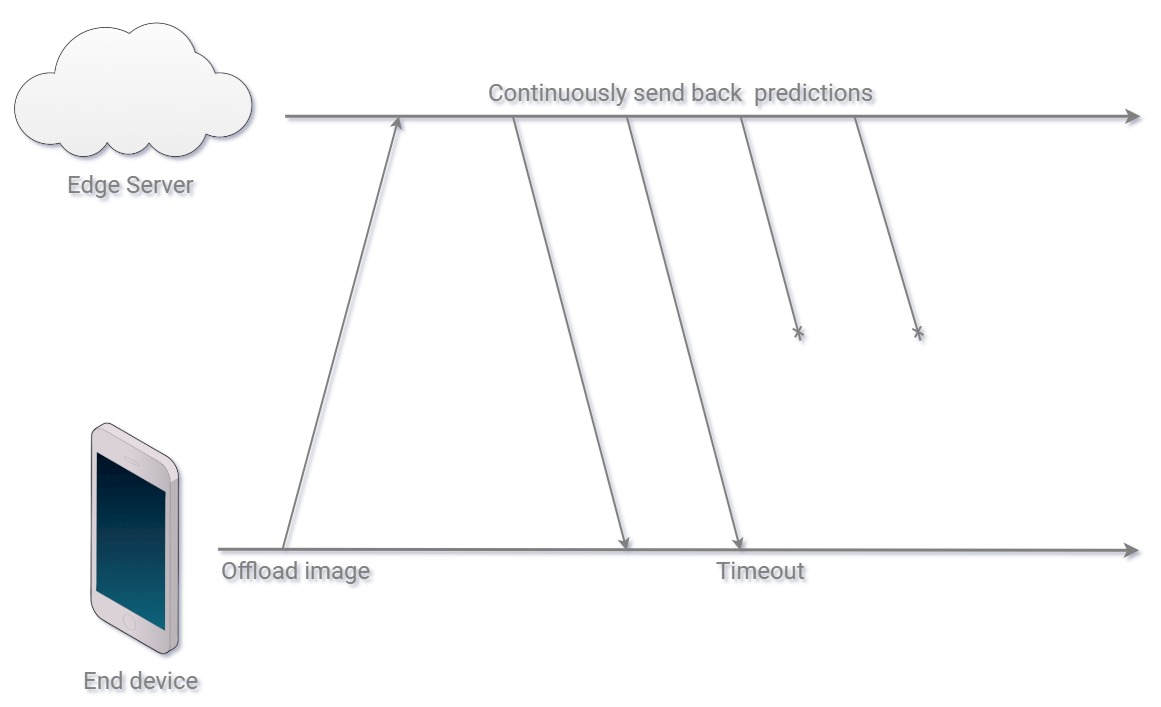
\includegraphics[width=\linewidth]{figures/models/timeline_timeout}}
	\caption[Offloading scheme]{offloading scheme}
	\label{fig:offloading-scheme}
\end{figure} 

\section{Implementation}

The offloading scheme is implemented as a client/server application using the \gls{python} Socket API. The client and server establishes a TCP socket. The client then loads a samples from the \gls{min100} validation set and sends it over the streaming protocol. The server preprocess the sample and runs the model inference. As prediction are obtained a thread is spawned to stream the results back to the end device. 

\section{Experimental Setup}

The client code is deployed on the NUC and server code on the Jetson TX2. The samples and intermediate predictions are timed an logged. 

\section{Results}



\subsection{Exit Score Analysis}

Having multiple predictions available give raise to the question, if we can use the additional information to improve model accuracy? An analysis of data have shown, that the score of an early exit is not always less than a later exit.
\begin{align*}
	s_{exit_{n}} \nless s_{exit_{n+1}}
\end{align*} 
\todo{How do I write the score of the prediction at an early exit is not always better than the later? And should I introduce the score and class label vectors earlier?}
Table \ref{tbl:latest-vs-max} show, that simply using the latest exit of the model is lightly better than using the highest scoring among all predictions, as uncertainty is introduced using earlier exits.  

\begin{longtabu}{>{\bfseries}X|X|X}
	\caption[]{} \label{tbl:latest-vs-max} \\
	\toprule
	\rowfont{\bfseries}
	Model & latest exit & max score   \tabularnewline
	\bottomrule
	\endfirsthead
	\multicolumn{3}{@{}l}{\textbf{\textcolor{black}{Table \ref{}:}} continued}\\
	\toprule
	\rowfont{\bfseries}
	Model & $Exit_N$ & max score    \tabularnewline
	\bottomrule
	\endhead % all the lines above this will be repeated on every page
	\bottomrule
	\multicolumn{3}{@{}l}{continued \ldots}\\
	\endfoot
	\hline
	\endlastfoot
	B-Resnet	& 0.8826	& 0.8794  \tabularnewline
	\hline
	B-DenseNet	& 0.8660 	& 0.8602 \tabularnewline 								
	\bottomrule
\end{longtabu}
Figure \ref{fig:exit-highscore} show the distribution of highest scoring exit given the amount of prediction received, and the distribution of samples correctly and incorrectly classified. Looking at the figure added uncertainty can be read directly from highest scoring exit is incorrect, where all predictions are received using the max score one must add the bars from all exits opposed to only using the red bar of $exit_N$. 

\begin{figure}
	\captionsetup[subfigure]{justification=centering}
	\centering
	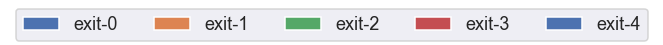
\includegraphics[width=.7\linewidth]{figures/edge/exit0-4_legend}
	\subfloat[B-ResNet]{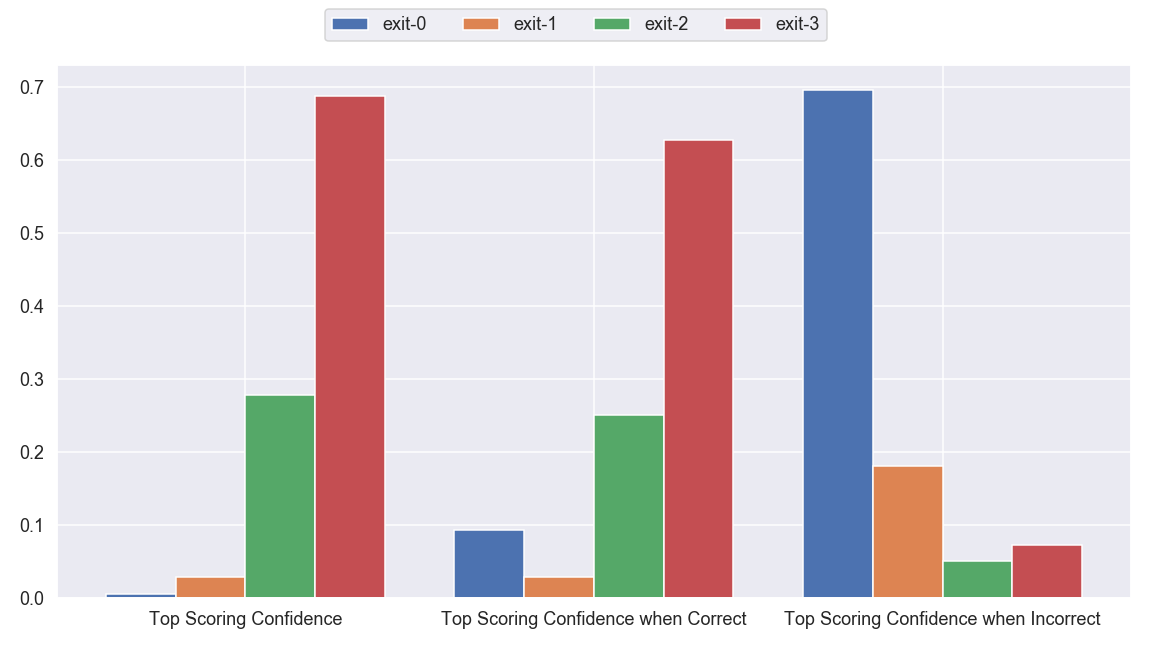
\includegraphics[width=.33\linewidth]{figures/edge/b-resnet_correctness}}
	\hfill
	\subfloat[B-DenseNet]{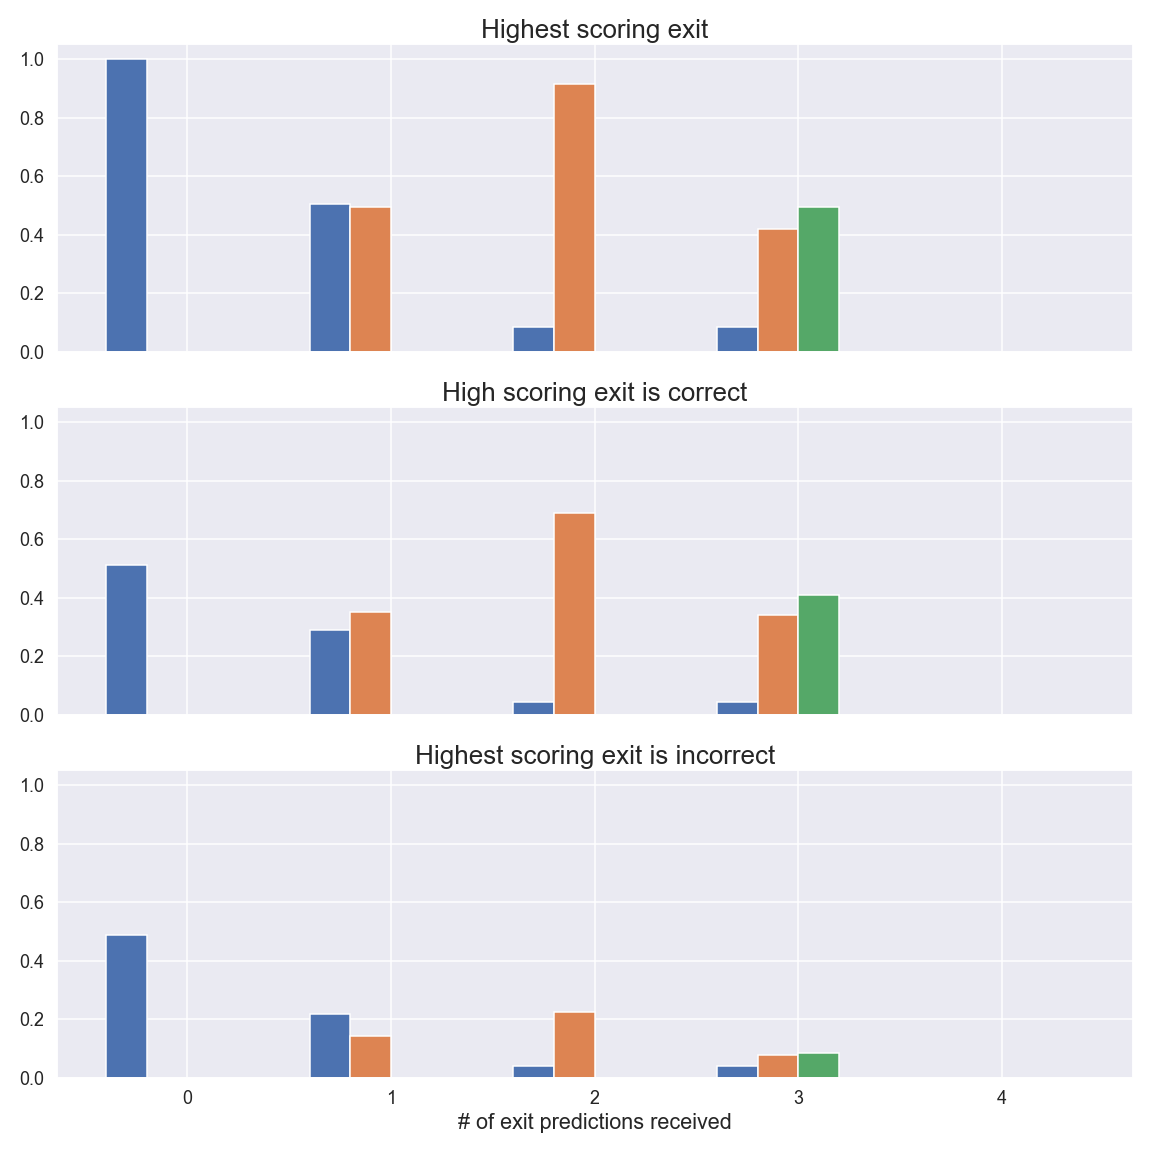
\includegraphics[width=.33\linewidth]{figures/edge/b-densenet_correctness}}
	\hfill
	\subfloat[MSDNet]{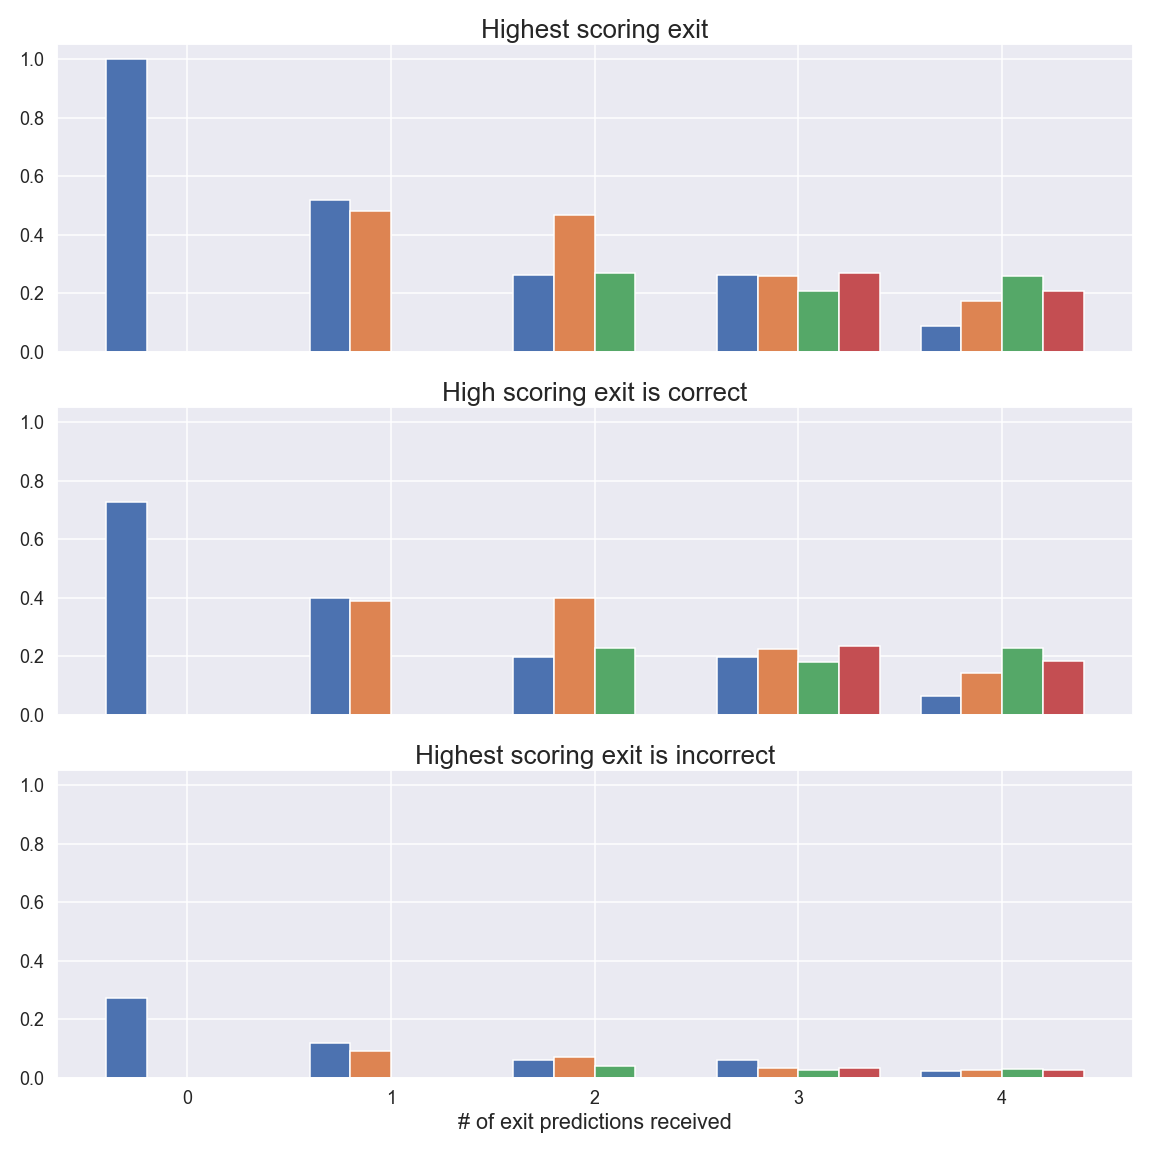
\includegraphics[width=.33\linewidth]{figures/edge/msdnet_correctness}}
	\caption[short text]{text}
	\label{fig:exit-highscore}
\end{figure}

Yet a study of samples revealed that in some cases an early exit correctly predicted a sample, which a later exit makes incorrect. An example is sample 57, where we denote a prediction vector $\mathbf{p}$ of binary values, where a 1 indicates a correct prediction and 0 the reverse. 
\begin{align*}
\mathbf{p}_{57}=
\begin{bmatrix}
exit_1 \\
exit_2 \\
exit_3 \\
exit_4
\end{bmatrix}
=
\begin{bmatrix}
1 \\
1 \\
0 \\
0
\end{bmatrix}
\end{align*}
Given this insight we define methods to combine the prediction information from multiple exit as efforts to improving the overall model accuracy. 

\subsection{Combining Prediction Information}

We define several proposals for using the additional predictions provided from the early exiting framework, with the purpose to improve the accuracy under time constraints. 

Each prediction contains two 5-dimensional vectors a class vector and a score vector. The class vector contains the sorted top-5 class labels. The score vector contains at the corresponding index the score associated with the class label. The scores are the output from the softmax classifier.
\begin{align*}
\mathbf{s}_{exit_n} = \begin{bmatrix}
s_{n,0} & s_{n,1} & s_{n,2} & s_{n,3} & s_{n,4}
\end{bmatrix} \\
\mathbf{c}_{exit_n} = \begin{bmatrix}
c_{n,0} & c_{n,1} & c_{n,2} & c_{n,3} & c_{n,4}
\end{bmatrix}
\end{align*}

To combine information from multiple predictions the vector must be expanded back to the original class space with $k$ classes. For the \gls{min100} $k=100$ expansion of the class vector $\mathbf{c}$ contains all class labels ordered and of course becomes identical for all exits.
\begin{align*}
\mathbf{c}_{exit_n}= 
\begin{bmatrix}
c_{n,0} & \dots & c_{n,4}
\end{bmatrix}_{1 \times 5}
\xrightarrow{expand} 
\mathbf{c} =
\begin{bmatrix}
0 & 1 & 2 & \dots & k-1
\end{bmatrix}_{1 \times k,\: k=100} 
\end{align*} 
For the score vector $\mathbf{s}$ we pad zero-value scores for all missing class labels.Thus, after expansion the vector only have non-zero values at the top-5 prediction indices.
\begin{align*}
\mathbf{s}_{exit_n} = 
\begin{bmatrix}
s_{n,0} & \dots s_{n,4}
\end{bmatrix}_{1 \times 5} 
\xrightarrow{expand}
\mathbf{s^*}_{exit_n}
\begin{bmatrix}
s_{n,0} & s_{n,1} & s_{n,2} &\dots & s_{n,k-1}
\end{bmatrix}_{1 \times k,\: k=100} 
\end{align*}
\todo{expansion to original class space, how to write that?}
\paragraph{Example: Expansion of a 10 class problem} 
\blockquote[]{	 	
	For this classification example, the number of classes $k=10$. From a prediction we get the two output vectors $\mathbf{c}$ and $\mathbf{s}$.
	\begin{align*}
	\mathbf{c} &= \begin{bmatrix}
	\phantom{0}0\phantom{.0} & \phantom{0}3\phantom{.0} & \phantom{0}6\phantom{.0} & \phantom{0}8\phantom{.0} & \phantom{0}9\phantom{.0}
	\end{bmatrix},\\
	\mathbf{s} &= \begin{bmatrix}
	0.80 & 0.10 & 0.05 & 0.03 & 0.01
	\end{bmatrix}
	\end{align*}
	We use or expansion method and two vectors $\mathbf{c}$ and $\mathbf{s}$ becomes expanded version two vectors $\mathbf{c^*}$ and $\mathbf{s^*}$.
	\begin{align*}
	\mathbf{c^*} &= \begin{bmatrix}
	\phantom{0}0\phantom{.0} & \phantom{0}1\phantom{.0} & \phantom{0}2\phantom{.0} & \phantom{0}3\phantom{.0} & \phantom{0}4\phantom{.0} & \phantom{0}5\phantom{.0} & \phantom{0}6\phantom{.0} & \phantom{0}7\phantom{.0} & \phantom{0}8\phantom{.0} & \phantom{0}9\phantom{.0}
	\end{bmatrix}_{1 \times 10},\\
	\mathbf{s^*} &= \begin{bmatrix}
	0.80 & 0.00 & 0.00 & 0.10 & 0.00 & 0.00 & 0.05 & 0.00 & 0.03 & 0.01
	\end{bmatrix}_{1 \times 10}
	\end{align*}
}
Given we receive $n$ prediction within the time frame, we can formulate $n \times k$ matrix S. 
%Each row contain the top-5 prediction from the corresponding exit and the columns contain the highest to lowest scoring of the top-5 prediction at all exits.
\begin{align*}
\mathbf{S}_{n,k} = \begin{bmatrix}
s^*_{0,0} & s^*_{0,1} & \dots  & s^*_{0,k-1} 	\\
s^*_{1,0} & s^*_{1,1} & \dots  & s^*_{1,k-1}	\\
\vdots 	& \vdots  & \ddots & \vdots 	\\
s^*_{n,0} & s^*_{n,1} & \dots  & s^*_{n,k-1}
\end{bmatrix}
\end{align*}      

\begin{description}
	
	\item[Lastest prediction] We define the method \emph{lastest prediction}, where we constraint ourselves to only use the most recent prediction $n$. We do not need to do any class expansion nor to formulate the matrix $\mathbf{S}$. We only need to consider the first index of the vector $\mathbf{c}_{exit_n}$. The class label becomes our prediction $p$.
	\begin{align*}
		p = \mathbf{c}_{exit_n,0}
	\end{align*}
	Equivalently we could expand our score vector to $\mathbf{s^*}$ and find the argument of the maxima.
	\begin{align*}
	p = \arg \max \mathbf{s^*}_{exit_n}	
	\end{align*}
	 Choosing the most confident prediction from the most recent result available, gives us the highest accuracy on average. However, we only use information form a single prediction, we might be able to formulate a mathematical function able to use information form multiple predictions to further improve the accuracy, as we have seen, that the later exit might make a correct prediction from an earlier exit incorrect. 
	 
	\item[Confidence (max)] This method is based on the naive assumption, that given a higher score, it will lead to a higher accuracy independent of the uncertainty of classifier at an earlier exits. We use class expansion and  formulation our score matrix $\mathbf{S}$. From $\mathbf{S}$ we find the prediction $p$ as the argument of the maxima.
	\begin{align*}
	p = \arg \max  \mathbf{S}
	\end{align*}
	
	\todo{How do I take first the row containing the max value, and then find the column/index of the maxium value?}
	Here we neglect the fact, that the later exits are in general more accurate and assume, that a higher confidence despite the exit leads to a correct prediction and we do not account for the uncertainty introduces be less accurate exits.

	\item[Confidence (add)] We define a method, that additive combines information from all available predictions and selects the highest scoring class. The score vector are be expanded to the class space and represented as a matrix. We sum all columns of $\mathbf{S}$ to a 1-dimensional vector $s_{sum}$ of length $k$. 
	
	\todo{how to sum column of matrix?}
	\begin{align*}
		\mathbf{s}_{sum} &= \sum_{i=0}^{k} \mathbf{S}_{n,i}, \text{for\:} n=0, 2, \dots, j\\ 
		&=	\begin{bmatrix}
		s^*_0 & s^*_1 \dots & s^*_{k-1}
		\end{bmatrix}_{1 \times k,\: k=100} 
	\end{align*}
	Our prediction becomes the argument of the maxima of $\mathbf{s}_{sum}$
	\begin{align*}
		p = \arg \max \mathbf{s}_{sum}
	\end{align*}
		

	\item[Confidence (add,weight)] Almost identical to \emph{confidence (add)}, but uses a weighted sum of all available exits to combine the information. Each exit are weighted to acknowledge the increasing accuracy as the predictions comes from a deeper exit in the model.  The weights can be represented by a column vector $\mathbf{w}$.
	\begin{align*}
		\mathbf{w}_{n} =
		\begin{bmatrix}
			w_0 &
			w_1 &
			\dots &
			w_n
		\end{bmatrix}^T
	\end{align*}
	The weights of row $n$ are multiplied all entries at row $n$ of $S$. Then we sum all columns of $\mathbf{S}$ to a 1-dimensional vector $s_{sum}$ of length $k$.  
	\begin{align*}
	\mathbf{s}_{ws} &= \sum_{i=0}^{k} w_n \cdot \mathbf{S}_{n,i}\\
	&= 		
	\begin{bmatrix}
	s_0 & s_1 \dots & s_{k-1}
	\end{bmatrix}_{1 \times k,\: k=100} 
	\end{align*}
	Our prediction becomes the argument of the maxima of $\mathbf{s}_{ws}$
	\begin{align*}
	p = \arg \max \mathbf{s}_{ws}
	\end{align*}
	
	\item[Score-margin (max)] We use the score-margin, defined in \ref{}, to find the best prediction among the available predictions. We do not need to expand our score vector nor to formulate the score matrix. Instead we define a $n$-dimensional column vector, where row $n$ represent the score-margin at the corresponding exit-$n$.  
	\begin{align*}
		\mathbf{s}_{sm} = \begin{bmatrix}
			\mathrm{ScoreMargin}(s_{0,0}, s_{0,1}) \\
			\mathrm{ScoreMargin}(s_{1,0}, s_{1,1}) \\
			\vdots \\
			\mathrm{ScoreMargin}(s_{n,0}, s_{n,1})
		\end{bmatrix}
	\end{align*}
	Our prediction becomes the argument of the maxima of the score-margin vector.
	\begin{align*}
		p = \arg \max \mathbf{s}_{sm}
	\end{align*}
	determines the score-margin between the two top-scoring predictions. We select the prediction from the exit with the highest score-margin. From the previous chapter, we know that the score-margin threshold gave a smaller proportion of incorrrectly exited samples at the small cost of samples, that could have been correctly classified using only highest scoring confidence.	
	\item[Score-margin (add)] Similarly we define a method, that determines the score-margin using the two highest scoring classes from each prediction and additive combines the informations.
	
	\item[Score-margin (add,weight)] Similarly we define a weighted sum version of the score-margin. 
\end{description}

\begin{figure}
	\captionsetup[subfigure]{justification=centering,farskip=1pt,captionskip=1pt}
	\centering
	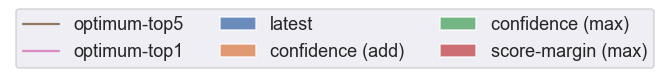
\includegraphics[width=.7\linewidth, keepaspectratio]{figures/edge/theoretical_score_combination_legend}
	\subfloat[subcaption]{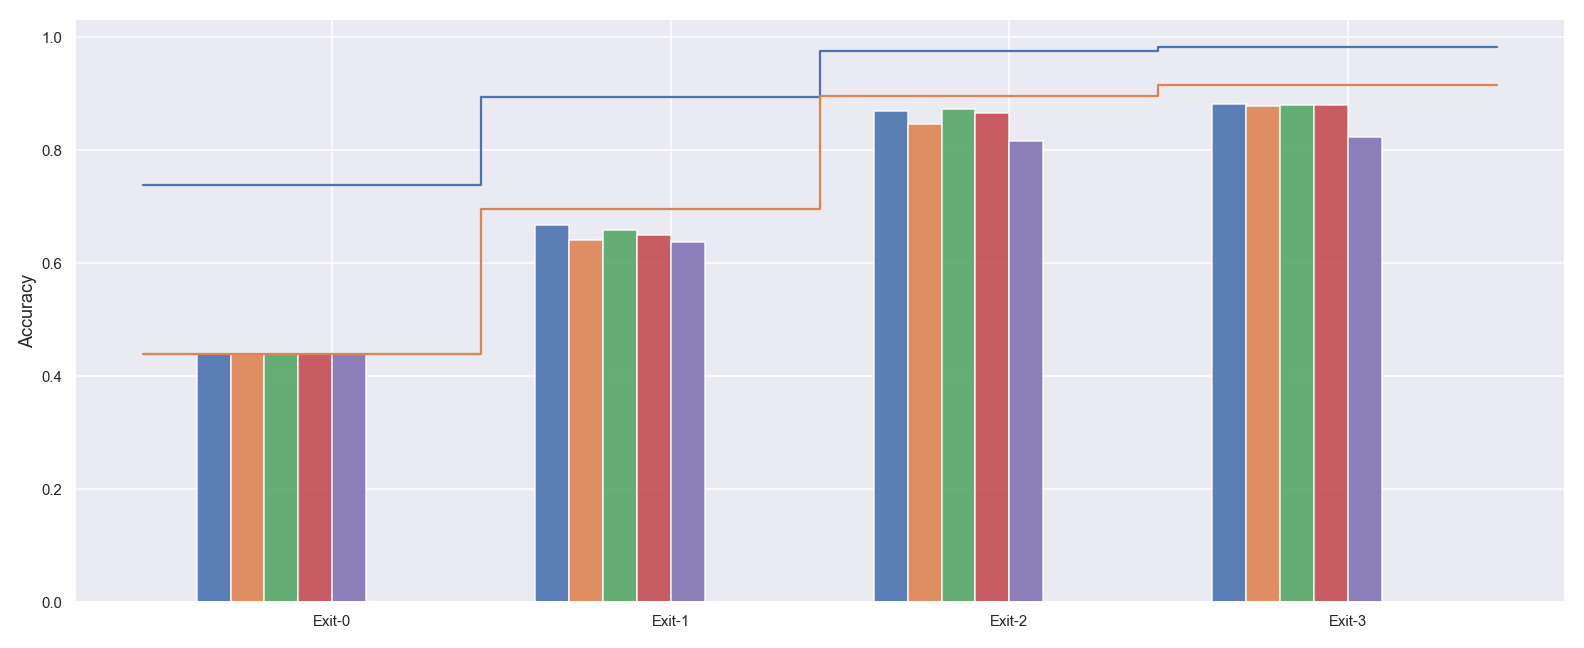
\includegraphics[width=.7\linewidth, height=.27\textheight, keepaspectratio]{figures/edge/b-resnet_theoretical_score_combinations}}
	\hfill
	\subfloat[subcaption]{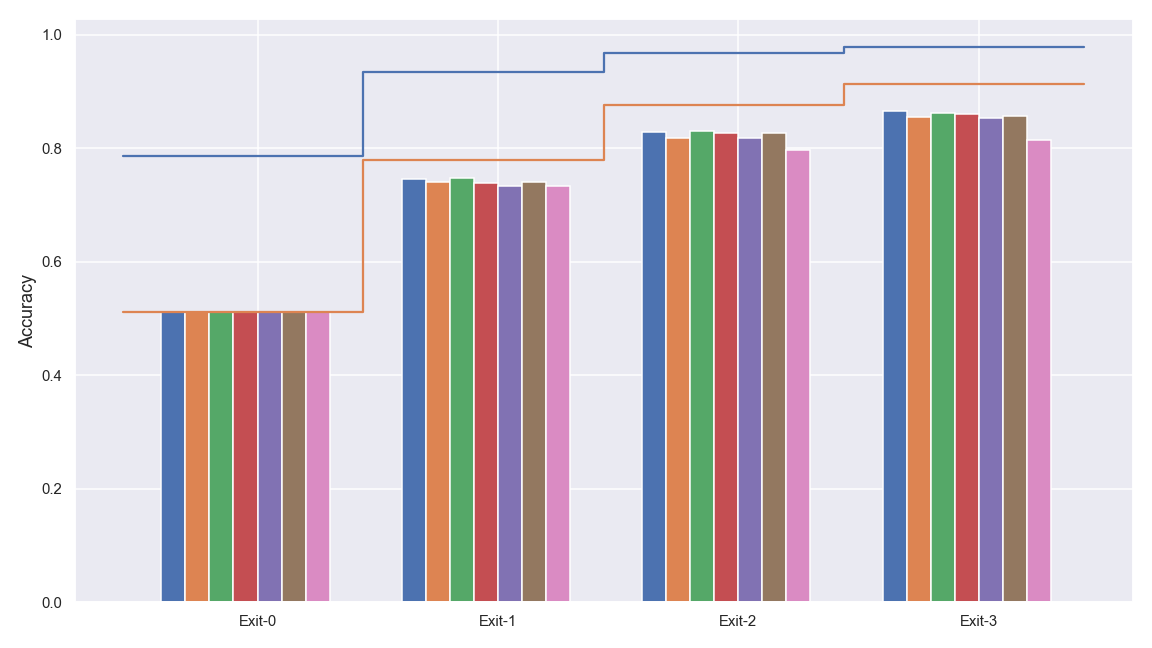
\includegraphics[width=.7\linewidth,height=.27\textheight, keepaspectratio]{figures/edge/b-densenet_theoretical_score_combinations}}
	\hfill
	\subfloat[subcaption]{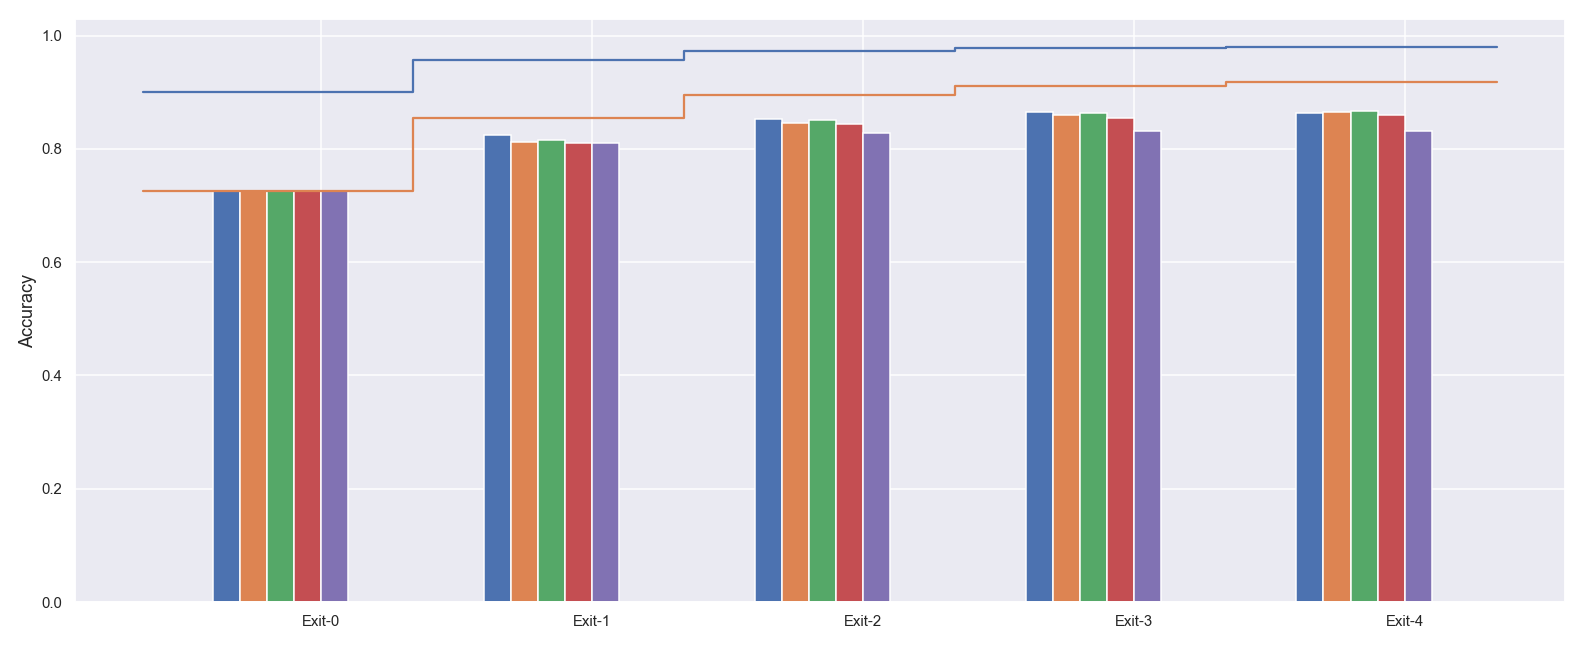
\includegraphics[width=.7\linewidth,height=.27\textheight, keepaspectratio]{figures/edge/msdnet_theoretical_score_combinations}}
	\caption[short text]{text}
	\label{fig:info-combi}
\end{figure}

The blue line optimum-top5 show the maximum achievable accuracy, if we were always able to pick the right class among the top5 predictions given the number of exit results received. The orange line optimum-top1 show the optimal line if, we were always able to pick the correct class among the top1 prediction given the number exit results received.

\subsection{Delay Constraint}

How far are we able to in inference process under different time constraints? 

\begin{figure}
	\centering
	\subfloat[]{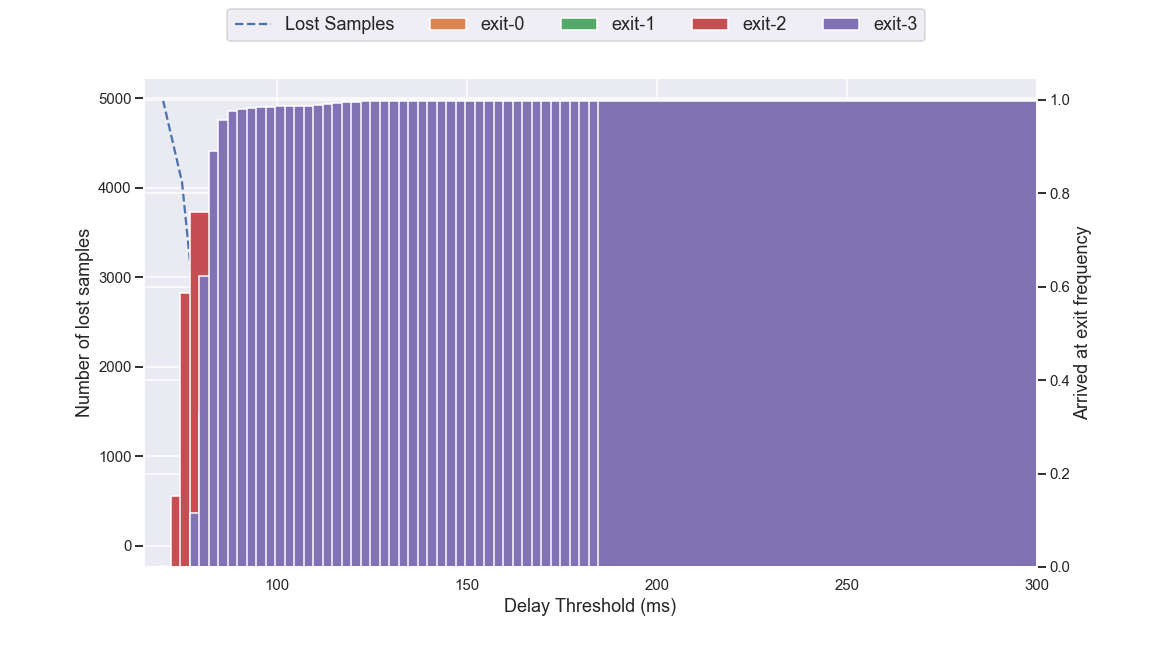
\includegraphics[width=.7\linewidth]{figures/edge/b-resnet_exit-reached}}
	\hfill
	\subfloat[]{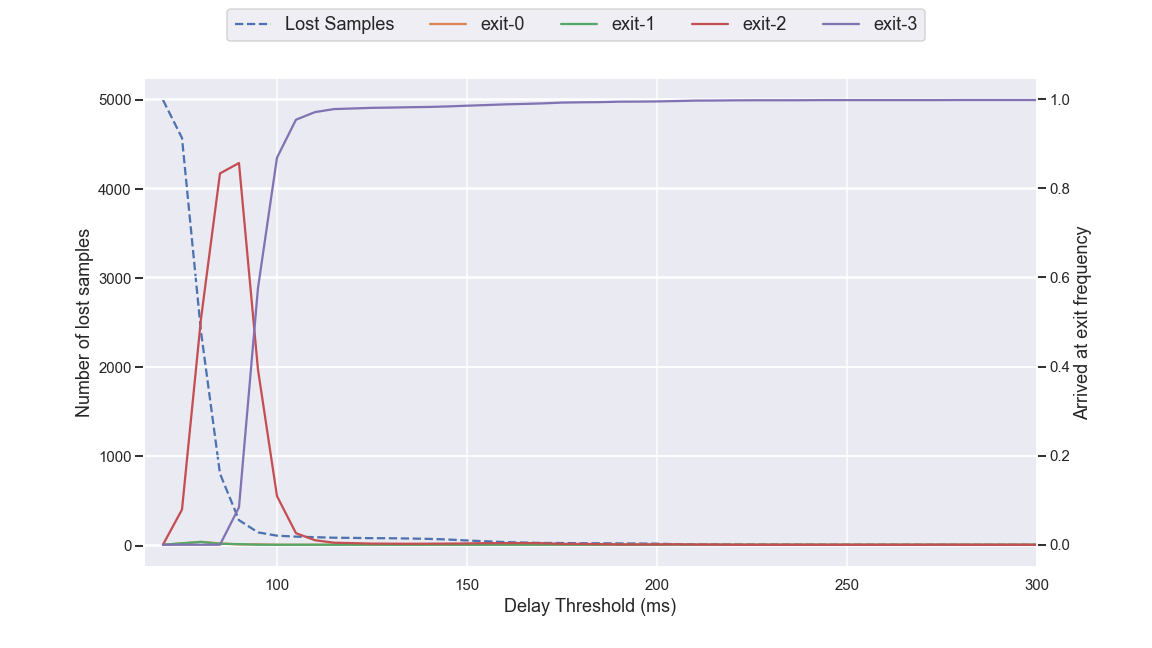
\includegraphics[width=.7\linewidth]{figures/edge/b-densenet_exit-reached}}
	\caption[short text]{text}
	\label{fig:exit-reached}
\end{figure}

\begin{figure}
	\centering
	\subfloat[subcaption]{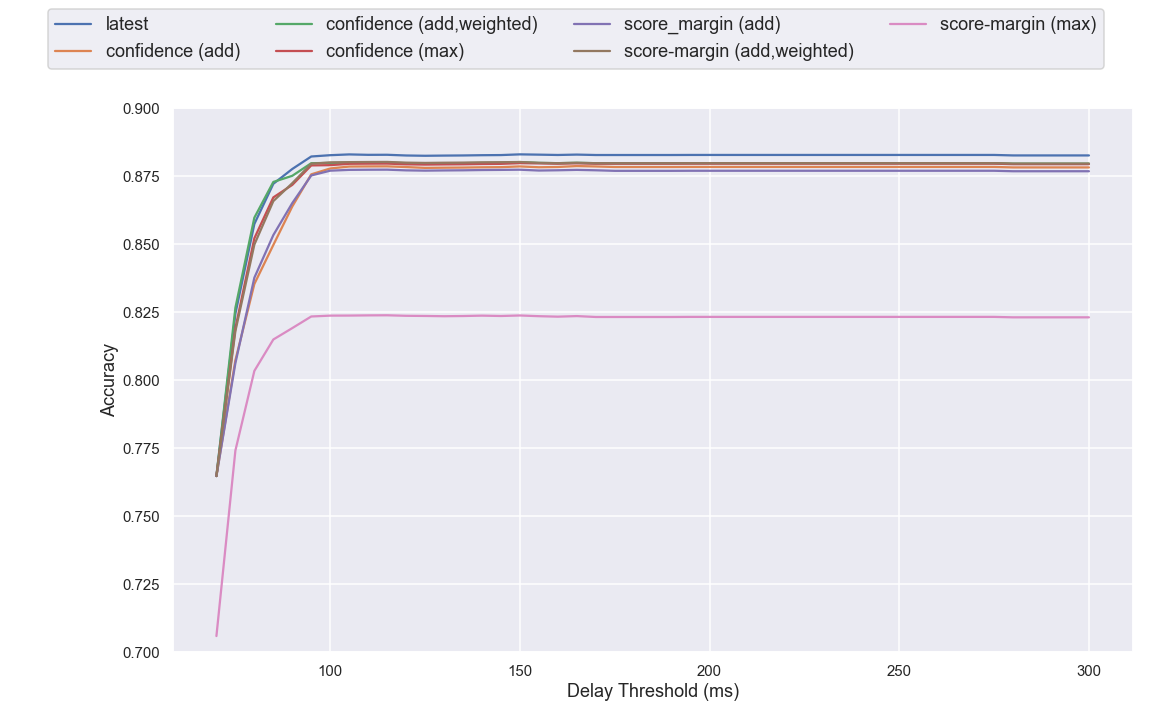
\includegraphics[width=\linewidth]{figures/edge/b-resnet_information-combination.png}}
	\hfill
	\subfloat[subcaption]{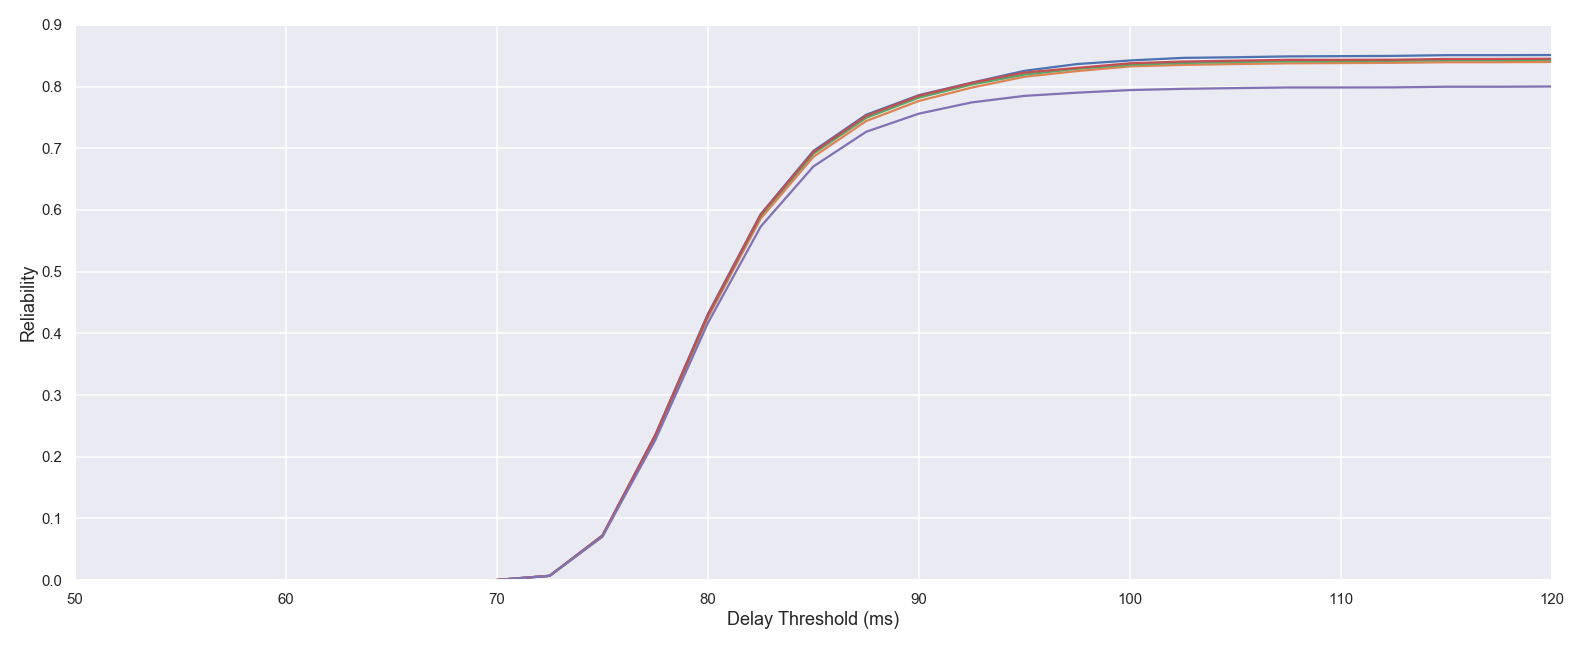
\includegraphics[width=\linewidth]{figures/edge/b-densenet_information-combination.png}}
	\caption[short text]{text}
	\label{fig:info-combi}
\end{figure}

Should I create hybrid combinations? Maybe only combine info from exit-0 and -1 and always let exit-2 and -3 have the final say if available? What if we can combine info from those two and omit the poor ones? 

\subsection{Transport Protocol} 

Offloading tasks over the network, irregardless fully or partially requires a transport protocol. The selection is typically a choice of either \gls{tcp} or \gls{udp}. \gls{tcp} is a reliable protocol, that guarantee no losses by retransmission of lost packets. \gls{udp} on the other hand is a best-effort protocol, that accept packets loss, thus not introducing retransmission communication overhead. 


Fully offloading \gls{jpeg} compressed images for classification require no losses for human-readability. Sending intermediate features of a \gls{dnn} may not be as intolerant to losses and might be able to function with the far more lightweight \gls{udp}. In current research literature the choice of \gls{tcp} seems given in advance.  

In this experiment the \gls{tcp} transmission time and retransmission rate is investigated under different communication environments. 

\begin{figure}
	\centering
	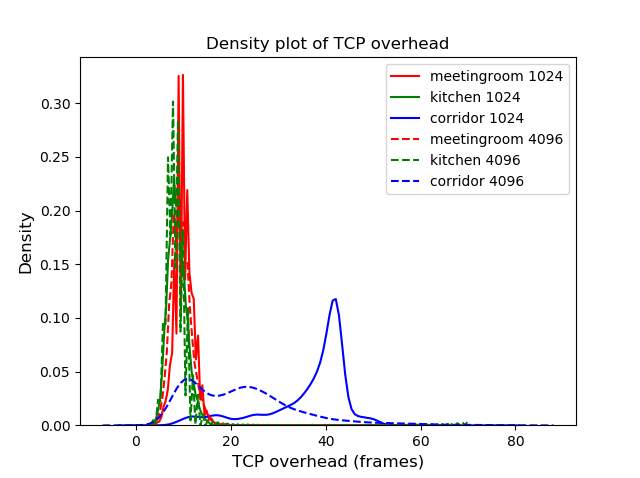
\includegraphics[width=\linewidth]{figures/tcp/tcpoverhead}
	\caption[TCP retransmission overhead]{TCP retransmission overhead}
\end{figure}

\section{Summary}

All offloading can lead to lost predictions under time stringent time constraints. If local processing is possible, then;

\begin{enumerate}
	\item \textbf{Collaborative Edge} where local inference of an early exit \gls{dnn} up to the first exit and then offload to the edge for remaining inference. The upside is, that running locally up to an exit, that should always be achievable guarantee a single prediction is available and mitigates lost prediction. The downsides are wasted idle time on edge server, as the slower end-device must do the most demanding early layers of the \gls{dnn}. Additionally offloading intermediate features that are typically larger than the original compressed images, hence the overall time becomes worse as communication is the bottleneck. This collaborative scheme require sophisticated compression of intermediate feature as in \cite{choi_near-lossless_2018} or a using \gls{bottlenet} layers.
	\item \textbf{Big/Little} A modified version of the Big/Little \gls{dnn}, where the end device offloads the compressed image to edge server and in parallel process a smaller and less accurate \gls{dnn} locally. The upside is, that the application can then always use the locally obtained prediction and choose to discard it as more accurate prediction arrives or combine information local and incoming predictions.
\end{enumerate}

